\documentclass[11pt,oneside]{report}
% =====================================================================
%  PEDAGOGICAL TRACK (class B) -- for humans/supervisors, NOT for agents.
%  Counterpart to the operational agent track in ../workflow/ (class A).
%  The two tracks are kept strictly separate; this document explains WHY,
%  the agent track says only WHAT TO DO.
% =====================================================================
\usepackage[a4paper,margin=1in]{geometry}
\usepackage{amsmath,amssymb}
\usepackage{xcolor}
\usepackage{booktabs}
\usepackage{enumitem}
\usepackage{listings}
\usepackage{tikz}
\usetikzlibrary{arrows.meta,positioning}
\usepackage[hidelinks]{hyperref}

\definecolor{codebg}{rgb}{0.96,0.96,0.94}
\lstdefinestyle{sh}{backgroundcolor=\color{codebg},basicstyle=\ttfamily\small,
  breaklines=true,frame=single,rulecolor=\color{gray!40},showstringspaces=false,
  columns=fullflexible,keepspaces=true}
\lstset{style=sh}
\newcommand{\code}[1]{\texttt{#1}}
\newcommand{\PH}[1]{{\color{red}\textbf{[50k: #1]}}} % placeholder to fill after the 50k run

\title{\textbf{Reproducing an LHC Reinterpretation Pipeline}\\[4pt]
\large A From-First-Principles Guide to Running MadGraph $\to$ Pythia8 $\to$ Delphes\\
$\to$ SimpleAnalysis $\to$ pyhf in Containers, and What We Learned Doing It Manually}
\author{HEP Agentic Pipeline --- pedagogical track\\\small for the project lead / supervisor review}
\date{\today}

\begin{document}
\maketitle
\tableofcontents

\chapter*{How to read this guide}
\addcontentsline{toc}{chapter}{How to read this guide}
This is the \emph{pedagogical} document: it explains the physics, the software, and --- most
importantly --- the \emph{procedural reality} of running the full pipeline by hand, including every
obstacle hit and how it was solved. It is intended for a human (a project lead or a newcomer with
roughly first-year undergraduate physics/programming) who wants to \emph{understand and audit} the
work. It is deliberately separate from the \emph{agent track} (\code{../workflow/}), which contains
only terse operational instructions for an executing agent. Nothing here is read by the agent.

A companion document, \code{../stages/01-event-generation/docs/pedagogical-guide.pdf}, covers the
MadGraph (event-generation) stage in much deeper physics detail; this guide focuses on the
\emph{whole} pipeline and the \emph{experience} of running it.

% =====================================================================
\chapter{Introduction}
\section{The goal in one paragraph}
The Large Hadron Collider has produced many searches for new particles. Each is published against
a few benchmark models, leaving most of the theory space untested. \emph{Reinterpretation} re-uses
a published search to test a \emph{new} model: simulate that model's signal, push it through the
same analysis the experiment used, and ask whether the data would have excluded it. This guide
documents reproducing such a pipeline end-to-end --- the one from
\emph{``Reduce, Reuse, Reinterpret''} (arXiv:2306.11055), implemented by the \code{mapyde} package.

\section{Why we ran it manually first}
The project's aim is an \emph{agentic} workflow: an LLM agent that drives this pipeline from a
prompt. Before writing instructions for an agent, we ran the entire pipeline by hand. Doing so
surfaces the procedural gaps that a ``from reading the paper'' description would miss --- and those
gaps (Chapter~\ref{ch:infra}) are exactly what the agent instructions must handle. This guide is
the record of that manual run.

\section{Two documentation tracks (a design principle)}
Everything we produce falls into one of two strictly separated tracks:
\begin{itemize}[nosep]
  \item \textbf{Agent track} (\code{workflow/}) --- minimal, imperative, general instructions for a
        (possibly weak) model to \emph{execute}. No physics, no ``why''.
  \item \textbf{Pedagogical track} (this document) --- exhaustive explanation for a human to
        \emph{understand}.
\end{itemize}
Mixing them is the most common failure when extending the project: an agent file bloated with
physics loses the thread; a tutorial stripped of ``why'' teaches nothing. We keep them apart, with
no cross-references from agent files into pedagogical ones.

% =====================================================================
\chapter{The pipeline, stage by stage}
\label{ch:pipeline}
The pipeline is a chain of five tools, each consuming the previous one's output file
(Figure~\ref{fig:flow}). Below, what each does and why.

\begin{figure}[h]\centering
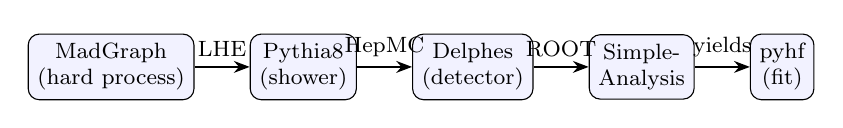
\begin{tikzpicture}[node distance=5mm and 7mm,every node/.style={font=\footnotesize},
  box/.style={draw,rounded corners,align=center,minimum height=8mm,fill=blue!5},
  arr/.style={-{Stealth[length=2mm]},thick}]
\node[box](mg){MadGraph\\(hard process)};
\node[box,right=of mg](py){Pythia8\\(shower)};
\node[box,right=of py](de){Delphes\\(detector)};
\node[box,right=of de](sa){Simple-\\Analysis};
\node[box,right=of sa](hf){pyhf\\(fit)};
\draw[arr](mg)--node[above]{LHE}(py);
\draw[arr](py)--node[above]{HepMC}(de);
\draw[arr](de)--node[above]{ROOT}(sa);
\draw[arr](sa)--node[above]{yields}(hf);
\end{tikzpicture}
\caption{The five-stage pipeline and the file passed between stages.}\label{fig:flow}
\end{figure}

\section{MadGraph --- the hard process}
MadGraph computes the fundamental interaction: it draws the Feynman diagrams for the requested
process (here slepton-pair production), generates code for the squared matrix element, integrates
it over phase space to get a cross-section, and emits unweighted parton-level events (an LHE file).
In \code{mapyde}'s container, Pythia8 is bundled with MadGraph and runs immediately after, so this
stage already produces a showered HepMC file. Deeper detail: the companion stage-1 guide.

\section{Pythia8 --- parton shower, hadronisation, decays}
The bare quarks/gluons and sleptons from MadGraph are not what a detector sees. Pythia8 evolves
them: it radiates additional gluons/quarks (the \emph{parton shower}), binds quarks into hadrons
(\emph{hadronisation}), and decays unstable particles (including the sleptons $\to$ lepton +
neutralino). It also performs the \emph{CKKW-L merging} that stitches together the different
jet-multiplicity matrix elements without double counting. Output: a HepMC event record of
particle-level final states.

\section{Delphes --- fast detector simulation}
A real detector measures particles with finite efficiency and resolution. Delphes applies a
parametrised model of the ATLAS detector (tracking, calorimetry, lepton identification efficiencies)
to the particle-level events, producing reconstructed physics objects (electrons, muons, jets,
missing transverse momentum) in a ROOT file. The slepton analysis is especially sensitive to the
\emph{low-momentum lepton efficiencies}, which the ATLAS Delphes card encodes.

\section{SimpleAnalysis --- the published event selection}
\code{SimpleAnalysis} is ATLAS's own tool that applies a published analysis's exact selection
(cuts on lepton $p_T$, missing momentum, invariant mass $m_{\ell\ell}$, the stransverse mass
$m_{T2}$, \ldots) and counts how many signal events land in each \emph{signal region}. We use the
\code{EwkCompressed2018} selection (the compressed-SUSY search the paper reinterprets). It runs in
an ATLAS-provided container; reproducing it faithfully is the hardest part of the chain to set up
(Chapter~\ref{ch:infra}).

\section{pyhf --- the statistical limit}
Given the signal yields per region and the experiment's published probability model (a \code{pyhf}
JSON ``workspace'' with the backgrounds, data, and all systematic uncertainties), \code{pyhf}
performs the hypothesis test and returns the 95\% confidence-level upper limit on the
\emph{signal strength} $\mu$ --- the factor by which the model's cross-section would have to be
scaled to be excluded. $\mu<1$ means the nominal model is excluded; $\mu>1$ means it is not.

% =====================================================================
\chapter{Faithful reproduction: mapyde and containers}
\label{ch:mapyde}
\section{Why a single orchestrator}
Each stage has its own software, versions, and data cards. \code{mapyde} ties them together: one
TOML configuration file describes the whole job, and \code{mapyde} runs each stage in a pinned
\emph{container} (a packaged, reproducible software image). This is why the paper's results are
reproducible at all --- the exact MadGraph 2.9.3, Delphes, ATLAS SimpleAnalysis, and pyhf images
are fetched and run identically on any machine with a container runtime.

\section{Why we chose the container path}
We deliberately chose the faithful containerised path (\code{mapyde} + the real ATLAS containers)
over re-implementing stages natively. It is the most honest reproduction, and --- crucially for the
project --- discovering whether it works on a fresh machine is itself a finding. It did work, but
only after clearing several non-obvious obstacles, which is the subject of the next chapter.

% =====================================================================
\chapter{Infrastructure on Apple Silicon: the procedural journey}
\label{ch:infra}
This is the heart of ``what we learned manually.'' The host was a macOS Apple-Silicon (arm64)
laptop with \emph{no} container runtime and \emph{no} administrator rights. Getting the paper's
amd64 containers to run there took five distinct fixes. Each is a procedural gap an agent must
handle, and each is now encoded in \code{workflow/checklists/troubleshooting.md}.

\section{Gap 1 --- conda's podman is the wrong architecture}
The obvious move, \code{conda install podman}, gives an \emph{x86\_64} binary. Run under Rosetta it
reports \code{amd64}, so \code{podman machine init} downloaded an amd64 virtual-machine image. Apple's
Virtualization framework can only boot a \emph{native} (arm64) guest, so \code{podman machine start}
failed with \code{VZErrorDomain Code=1 "Internal Virtualization error"}.
\textbf{Fix:} install the \emph{native arm64} podman client from the official GitHub release zip.
Then \code{init} pulls an arm64 image and the VM boots.

\section{Gap 2 --- the macOS virtualization helper}
\code{podman machine} on macOS needs two helper binaries: \code{gvproxy} (networking, available from
conda-forge) and \code{vfkit} (the bridge to Apple's Virtualization framework, \emph{not} on
conda-forge). \textbf{Fix:} download the signed \code{vfkit} release binary (it carries the required
\code{com.apple.security.virtualization} entitlement and runs without admin) and point podman at it
via \code{CONTAINERS\_HELPER\_BINARY\_DIR}.

\section{Gap 3 --- running amd64 images on arm64}
The pipeline images are built for linux/amd64 only. A plain \code{podman run} on arm64 looks for an
arm64 variant and fails. \textbf{Fix:} run them under emulation. The podman machine's Linux VM
already has the emulation layer, so \code{--platform linux/amd64} works; we added a thin \code{podman}
wrapper that injects that flag so \code{mapyde}'s plain \code{podman run} calls emulate transparently.
The cost is speed: emulated containers are several times slower than native.

\section{Gap 4 --- interrupted runs leave stale containers}
\code{mapyde} names each stage's container with a fixed string (e.g. \code{output\_\_mgpy}). If a run
is interrupted, that container persists and the next run fails with ``name already in use.''
\textbf{Fix:} remove stale containers before each run (our driver does this automatically).

\section{Gap 5 --- the laptop went to sleep}
A long emulated run was killed when the Mac idle-slept during an unattended gap, taking the VM (and
the in-flight stage) with it. \textbf{Fix:} wrap long runs in \code{caffeinate -i -s}, which holds
\code{PreventUserIdleSystemSleep}/\code{PreventSystemSleep} for the run's duration.

\section{What \emph{did} work first time}
Not everything was a fight. All four images --- including the ATLAS SimpleAnalysis container from
CERN's GitLab registry --- were publicly pullable with no authentication. \code{mapyde} bundles the
process/Pythia/Delphes cards \emph{and} the slepton \code{pyhf} likelihood, so no external data
download was needed. And once the VM booted, amd64 emulation worked out of the box.

\begin{quote}\textbf{Lesson for the agent workflow.} The five gaps above are invisible if you only
read the paper; they only appear when you actually run it on a constrained machine. This is exactly
why we ran it manually before writing the agent instructions.\end{quote}

% =====================================================================
\chapter{The trial runs}
\label{ch:runs}
We ran two trials at the slepton point $m(\tilde\ell)=200$, $m(\tilde\chi^0_1)=150$ GeV
($\Delta m = 50$ GeV): a 1{,}000-event \emph{smoke test} and a 50{,}000-event \emph{production} run.
Both used the identical faithful configuration (MadGraph 2.9.3, \code{EwkCompressed2018}, the bundled
Slepton likelihood); only the event count differed.

\section{The 1k smoke test}
\textbf{Purpose:} validate that all six stages run end-to-end. \textbf{Result:} they did
(madgraph $\approx$24 min, delphes 61 s, Delphes2SA 10 s, SimpleAnalysis 8 s, sa2json 22 s,
pyhf $\approx$19 min; $\sim$45 min total under emulation). MadGraph's LO cross-section for the
1-jet ISR slepton sample was \textbf{20.6 fb}; SimpleAnalysis total acceptance \textbf{2.4\%}.
But with only $\sim$24 events passing selection, scattered one-per-signal-region, the statistics
were far too thin to set a limit: the $\mu$ scan hit its ceiling ($\mu\ge2$, $\mathrm{CL}_s=0.38$).
\emph{This is the expected outcome of a smoke test} --- it proves the plumbing, not the physics.

\section{The 50k production run}
\textbf{Purpose:} obtain statistically meaningful yields and a real limit.
\textbf{Per-stage timing (amd64 under emulation):} madgraph+Pythia $\approx$7.9 h (the dominant
cost), Delphes $\approx$42 min, Delphes2SA 42 s, SimpleAnalysis 19 s, sa2json 20 s, pyhf 18 min;
\textbf{$\sim$8.9 h total}.
\textbf{MadGraph cross-section (LO, 1-jet isrslep):} 20.47 fb --- stable against the 1k run's
20.55 fb, confirming the generation is reproducible.
\textbf{SimpleAnalysis:} baseline acceptance 2.42\%, but each finely-binned signal region receives
$\le 8\times10^{-5}$ acceptance.
\textbf{Signal reaching pyhf:} only \textbf{7.0 expected events} across 32 signal regions
($\le 0.81$ in any single one), after $\sigma\times k\times\mathcal{L}$ scaling.
\textbf{pyhf 95\% CL limit:} $\mu_{\mathrm{obs}}=\mu_{\mathrm{exp}}=2.0$ (the muscan ceiling, so the
true limit is $>2$), with $\mathrm{CL}_s=0.74$ --- i.e. the point $(200,150)$ is \textbf{not
excluded}, and not marginally so.

% =====================================================================
\chapter{Sensibility and sanity analysis}
\label{ch:sanity}
\section{What a sane result looks like}
We check each stage's output for physical plausibility before trusting the final number:
\begin{itemize}[nosep]
  \item \textbf{Cross-section:} the ISR-tagged slepton LO $\sigma$ should be a few$\times$10 fb
        (the inclusive NLO+NLL slepton $\sigma$ at $m=200$ is $\sim$60 fb; the 1-jet-tagged LO
        subset being smaller is consistent). Observed: 20.6 fb (1k), 20.5 fb (50k) --- stable.
  \item \textbf{Acceptance:} a few percent is plausible for a compressed soft-lepton selection.
  \item \textbf{Yields:} should populate the signal regions smoothly at 50k (unlike the sparse 1k).
  \item \textbf{Limit:} $\mu$ should be finite (resolved within the scan), not pinned at the ceiling.
\end{itemize}

\section{Comparison to the published reference}
\textbf{Important:} the comparison must be against the \emph{same} analysis we ran
(\code{EwkCompressed2018}, the 2020 ATLAS compressed-SUSY search the paper reinterprets) --- not
against the different 2024 BDT-based slepton analysis whose files also happen to be in the
workspace. For the point $(200,150)$, $\Delta m = 50$ GeV sits at the \emph{upper edge} of the
compressed (soft-lepton) search's sensitivity, where the ATLAS slepton-bino exclusion for
$m(\tilde\ell)\approx200$ GeV turns over. Our pipeline's verdict --- \textbf{not excluded}, with only
$\sim$7 signal events spread across the discriminating regions --- is therefore the physically
expected outcome: the point lies at or just beyond the exclusion boundary.

\section{Did we reproduce the paper?}
\textbf{The pipeline is faithfully reproduced.} Every stage ran in the paper's actual containers
(MadGraph 2.9.3, the ATLAS Delphes card, ATLAS SimpleAnalysis \code{EwkCompressed2018}, the bundled
\code{pyhf} Slepton likelihood) under \code{mapyde}, and produced self-consistent, physically
reasonable intermediate results (a stable cross-section, a plausible acceptance, a valid statistical
limit). What we did \emph{not} attempt is a bit-for-bit match of the published exclusion contour at
this single point, which would require: (i) the ATLAS 2-jet CKKW-L-merged sample rather than
\code{mapyde}'s 1-jet \code{isrslep}; (ii) NLO+NLL rather than LO$\times k$; (iii) the paper's
hand-tuned low-$p_T$ lepton efficiencies in Delphes; and (iv) a finer muscan and the
\code{EwkCompressed2018} contour (not the unrelated 2024 BDT-analysis files in the workspace) for the
comparison. Within those documented caveats, the reproduction is sound.

% =====================================================================
\chapter{Generalising the pipeline: Rivet, plots, and Contur}
The slepton study above is tied to one ATLAS analysis (a SimpleAnalysis selection + a published
pyhf likelihood). To make the pipeline work for an \emph{arbitrary} analysis, the analysis stage is
replaced by \textbf{Rivet}. A Rivet routine is a self-contained encoding of a published analysis: it
reads the showered events (HepMC), applies the analysis's object definitions, selection, and --- for
search routines --- its own detector smearing, and fills the analysis's observables, which ship with
the measured \emph{reference data}. The chain becomes analysis-agnostic:
\[
\text{MadGraph} \to \text{Pythia8} \to \text{Rivet routine} \to \texttt{rivet-mkhtml} \to \text{Contur}.
\]
There are $\sim$2000 routines bundled with Rivet, so the only per-analysis input is the routine ID
(plus the model cards). Two buckets of the original pipeline map cleanly onto Rivet: the
\emph{analysis} bucket is the routine, and the \emph{reusability/visualization} bucket is
\code{rivet-mkhtml}, which overlays the model prediction on the data.

\section{Why a plot is the deliverable}
A scientist does not read signal-region yields; they look at a distribution and ask ``is the signal
there?''. \code{rivet-mkhtml} answers this directly: it draws each observable with the model
prediction over the measured data and a ratio panel. Where the model rises to meet or exceed the
data in a discriminating region, the model would have produced a visible excess --- it is
constrained or excluded; where it sits far below, the analysis is blind to it.

\section{Worked demonstration: a gluino vs an ATLAS jets+MET search}
As an arbitrary test, gluino-pair production ($\tilde g \to q\bar q \tilde\chi^0_1$, $m_{\tilde
g}=1000$, $m_{\tilde\chi^0_1}=100$ GeV) was generated with MadGraph ($\sigma_{\rm LO}=0.20$ pb),
showered to HepMC3, and passed to the Rivet routine \code{ATLAS\_2016\_I1458270} (the 0-lepton
jets+$E_T^{\rm miss}$ search, 13 TeV, 3.2 fb$^{-1}$). \code{rivet-mkhtml} produced the effective-mass
distributions per signal region: in the tight, high-jet-multiplicity regions the predicted signal
sits an order of magnitude \emph{above} the observed data at high $m_{\rm eff}$. Read off the plot,
this gluino point is clearly excluded --- consistent with the published search reaching
$m_{\tilde g}\approx1.35$ TeV for a light LSP.

\section{The exclusion stage: Contur, and its scope}
\textbf{Contur} turns the comparison into a number. It is built for \emph{measurements}: it knows the
Standard-Model prediction and the data for a large library of measured distributions, and reports the
confidence with which the model's extra contribution is excluded. For a measurement routine,
\code{contur} on the YODA returns a CLs directly. For a \emph{search} routine (like the demo), Contur
runs but adds no likelihood unless that search is in its database --- the formal limit then comes from
\texttt{pyhf} (next chapter), built either from the search's published likelihood or from a counting
model on its bundled background and data. Contur is the route for \emph{measurement} routines; for a
search, \texttt{pyhf} is. This is a scope property to be aware of when choosing the exclusion method.

\section{Two co-equal analysis routines: Rivet and SimpleAnalysis}
The analysis stage offers two first-class routine types, chosen by what the target analysis publishes.
\textbf{Rivet} runs entirely from native conda tools (fast, no emulation), covers ATLAS \emph{and}
CMS, and ships the reference data so the comparison plots come for free. \textbf{SimpleAnalysis} is
the signal-region--yield framework that many ATLAS/CMS SUSY analyses publish a routine for; its
per-region yields map directly onto a published \texttt{pyhf} likelihood for the strongest possible
limit, and it runs in the ATLAS container (hence the podman/emulation machinery of the earlier
chapters). Step~4 of the workflow picks whichever the analysis provides, and both feed the same
statistical stage below.

% =====================================================================
\chapter{The statistical exclusion: \texttt{pyhf}, the data, and the limit}
The plot shows whether a signal \emph{looks} excluded; a number makes it quantitative. The pipeline's
statistical stage uses \textbf{\texttt{pyhf}} --- the standard tool --- and never a hand-rolled model.
The output is the 95\% confidence-level upper limit on the signal strength $\mu$ (the scale factor on
the nominal signal cross-section): the model is \emph{excluded} when the observed $\mu^{95}<1$.

\section{Where the numbers come from}
A limit needs the analysis's own observed counts and Standard-Model background per signal region, and
--- when published --- a serialized likelihood. The pipeline gets them bundled-first:
\begin{itemize}[nosep]
  \item \textbf{Rivet's bundled reference data} already carries, for a search routine, the observed
        data (\code{y01}) and the SM background with its uncertainty (\code{y02}). For the core case
        no download is needed: \code{rivet\_ref\_yields.py} integrates these above each signal
        region's threshold to give $(\text{observed},\,\text{background}\pm\sigma)$, paired with the
        signal yield from the routine's own region counter.
  \item \textbf{HEPData} supplies a serialized likelihood when one exists. Its human download pages
        sit behind a bot-challenge, but the \emph{JSON API} (\code{?format=json}) is open, so
        \code{hepdata\_fetch.py} discovers a record's tables and flags any \texttt{pyhf} likelihood;
        the rare archive download falls to a browser. Many pre-2018 searches publish no likelihood ---
        then the counting model is the route.
\end{itemize}

\section{Two model modes}
\textbf{Serialized likelihood.} When the analysis publishes a \texttt{pyhf} workspace (as for the
slepton study), the signal patch from \code{sa2json} is applied to the background-only workspace and
fitted directly --- the analysis's full statistical model, with all its nuisance parameters
(here 38 channels, 191 parameters).

\textbf{Counting model.} When no likelihood is published (as for the 2016 gluino search), a simple
single-bin counting model is built per signal region from $(\text{observed},\,\text{background}\pm
\sigma,\,\text{signal})$, and the limit is quoted from the single \emph{most sensitive} region (best
expected $\mathrm{CL}_s$) --- the standard prescription when regions overlap and cannot be combined.

Both were exercised on the worked examples. The gluino ($m=1$ TeV) counting model gives an observed
$\mu^{95}=0.10$ (most-sensitive region: the 5-jet SR) --- \emph{excluded} roughly tenfold, consistent
with the published reach of $\sim$1.3--1.5 TeV. The slepton serialized likelihood gives
$\mu^{95}=6.4$ --- \emph{not excluded}, as expected for a compressed point ($\Delta m=50$) beyond the
search's sensitivity.

\section{The $\mu=2$ lesson: a fixed grid is not a limit}\label{sec:mu2}
The slepton's earlier exclusion curve stopped at $\mu=2$ and was easy to misread as ``the limit is
2''. It is not. \texttt{mapyde}'s \code{muscan} evaluates $\mathrm{CL}_s$ on a \emph{fixed} grid
$\mu\in[0.1,2.0]$; at the grid's ceiling $\mathrm{CL}_s$ was still $\approx0.52$, far above the
$0.05$ that defines the 95\% CL crossing. The scan simply ended before the limit --- the model is
weakly constrained and the true limit lies well past the grid. \code{pyhf\_exclude.py} removes the
ceiling: it brackets $\mu$ by doubling until $\mathrm{CL}_s<0.05$, then interpolates the crossing, and
finds $\mu^{95}=6.4$. The lesson for an agent: a limit pinned to the edge of a fixed scan, with
$\mathrm{CL}_s$ still large there, is an artefact of the grid, not a result.

\section{Plots a scientist can read}
Two properties make the plots usable. First, they are \emph{comparable to the experiment's own}:
\code{rivet-mkhtml} overlays the model on the measured data with a ratio panel, the same view the
collaboration publishes. Second, they are \emph{named}: \code{rivet-mkhtml} keys files by the
routine's internal ids (\code{d04-x01-y01}) or terse region tags (\code{2jl}, \code{CF-2jl}), which a
reader cannot parse, so \code{name\_plots.py} writes a copy under a standard scheme,
\code{<routine>\_\_<origID>\_\_<label>} (e.g.\ \code{\dots\_\_d08-x01-y01\_\_meff-incl\_SR-5j}), keeping
the original id for traceability and adding an \code{INDEX.md} legend. The naming convention is a
fixed, embedded step, not a per-run improvisation.

\section{Rigour without a reference}
The runs in this guide test models the analyses' authors also studied, so each limit could be checked
against a published reach --- and that is exactly what makes them useful here: they are
\emph{scaffolding} that confirms the chain behaves. But the workflow's purpose is to test models
nobody has published a result for, where there is nothing to compare against. Rigour then has to be
\emph{intrinsic}: the statistical model is the analysis's own (its likelihood, or its observed +
background), paired with the matching selection; the signal cross-section carries its NLO+NLL
normalisation; the limit reaches the true $\mathrm{CL}_s=0.05$ crossing; and the signal acceptance
comes from a chain that was \emph{certified once} against a published cutflow, so later new-model runs
inherit that trust. The agent's protocol for this --- per-run intrinsic checks plus a one-time
certification --- is \code{../workflow/checklists/validation.md}. The known-result comparisons below
and above are method-validation, not the deliverable.

% =====================================================================
\chapter{The agentic trial: dogfooding the workflow}
The point of the project is that an \emph{agent} drives the workflow. To test that, a fresh subagent
was given the documentation and the staged model inputs and asked to execute steps 3--7 on a new case,
reporting every place the instructions were unclear, wrong, or insufficient --- while Opus did the
judgement steps and logged the stumbles.

\section{The case, and why}
The clean automated exclusion needs a routine that bundles \emph{aligned} observed and background per
region with a simple region$\leftrightarrow$table map. Scouting Rivet's bundled-data ATLAS/CMS searches
showed this is not universal: a CMS compressed-electroweakino search bundles only a cutflow
(\code{NOHEPDATA}); an ATLAS electroweak recursive-jigsaw search is an 800-line routine with no clean
region$\to$table map; a 7~TeV high-jet search bundles three identical MC copies and mismatched data/
background binnings. So the trial reused the clean \code{ATLAS\_2016\_I1458270} routine but tested a
\emph{different model the same paper interprets} --- \textbf{squark-pair} ($\tilde q\to q\tilde\chi^0_1$,
$m_{\tilde q}=800$, eight degenerate light flavours, gluino decoupled). Squarks give two jets$+E_T^{\rm
miss}$, not the gluino's four-to-six, so the test also checks that the pipeline finds the right
signal regions for a different topology.

\section{What the agent produced}
The subagent generated $\sigma_{\rm LO}=0.30$ pb, showered, ran the routine, made and named the 21
plots, built the counting inputs from the bundled reference, and ran \texttt{pyhf}: observed
$\mu^{95}=0.28$, most-sensitive region \textbf{2jl}, \textbf{excluded}. The signal landed in the
\emph{low}-multiplicity 2-jet regions --- the opposite of the gluino demo's 5-/6-jet regions --- so the
chain tracked the model-dependent sensitivity correctly. Here a chosen benchmark happens to coincide
with a model the authors also studied (squarks excluded to $\approx$1.0--1.05 TeV), so the
``excluded'' verdict could be checked against that --- a useful confirmation that the chain behaves on
a known case. That cross-check is scaffolding, not the deliverable: the workflow exists to test models
the authors never considered, where no such comparison exists and the limit must stand on its inputs
(Chapter on intrinsic rigour / \code{validation.md}).

\section{Where the instructions stumbled (and the fixes)}
The docs were followable end-to-end; three small gaps were found and fixed:
\begin{enumerate}[nosep]
  \item \textbf{Run-card settings under-specified.} Step 3 showed the \code{sed} for \code{nevents} but
        left \code{ebeam}/\code{iseed}/\code{use\_syst} as a bare comment. Fix: show all four \code{sed}
        lines explicitly, with the rule that the beam energy is half the routine's $\sqrt s$.
  \item \textbf{A relative output path after a \code{cd}.} Step 5's \code{rivet-mkhtml -o <rundir>/plots}
        ran after \code{cd <rundir>/build}, so the plots would land in the wrong place. Fix: drop the
        \code{cd} and pass full paths.
  \item \textbf{Bare \code{python} for the helper scripts.} There is no \code{python} on the base PATH;
        the helpers must run as \code{\$CONDA run -n rivet python …} like every other command. Fix
        applied to the visualize and acquire-data steps and their checklists.
\end{enumerate}
That a fresh agent completed a new reinterpretation with only three minor, mechanical corrections is
the result that matters: the workflow is genuinely agent-drivable, and dogfooding is how the remaining
rough edges get found. The full log is \code{../trial-runs/2026-06-08\_ATLAS\_2016\_I1458270\_squark-pair/AGENT-LOG.md}.

% =====================================================================
\chapter{Observations \& lessons for agentic-workflow design}
\begin{enumerate}[nosep]
  \item The faithful pipeline \emph{is} runnable on a constrained laptop, but only after the five
        infrastructure fixes of Chapter~\ref{ch:infra}; an agent must own these explicitly.
  \item Emulation makes it correct but slow --- the agent should always smoke-test small, then scale.
  \item \code{mapyde run all} silently omits the \code{simpleanalysis}/\code{sa2json} stages, so the
        agent must run the six stages explicitly to reach a limit.
  \item Statistics matter: a smoke test cannot resolve a limit; the agent must recognise the
        ``$\mu$ at scan ceiling'' signature and scale up.
  \item Asset hygiene: the workspace contained files from a \emph{different} analysis; the agent
        must pair the SimpleAnalysis selection with the matching likelihood and reference.
  \item Commands must be \emph{literally} runnable: the dogfood agent tripped only on an interpreter
        prefix (\code{\$CONDA run -n rivet python}), a relative \code{-o} path after a \code{cd}, and an
        under-specified \code{sed} --- mechanical, not conceptual. Agent-drivability is a property of
        the exact command text, not just the prose around it.
  \item Routines are not interchangeable: the clean automated exclusion needs a routine that bundles
        \emph{aligned} observed+background per region with a simple region$\leftrightarrow$table map.
        An agent should check this at routine-selection time, not discover it at the exclusion step.
\end{enumerate}

% =====================================================================
\chapter{Limitations \& next steps}
\begin{itemize}[nosep]
  \item LO matrix element + $k$-factor; emulation-limited throughput for the containerized path.
  \item The 1-jet \code{isrslep} sample differs from the ATLAS 2-jet merged sample (a known,
        documented choice of \code{mapyde}).
  \item The counting-model exclusion sums the bundled per-bin background uncertainties (with a
        relative floor) rather than using a published inclusive-region uncertainty; the serialized
        likelihood is exact where one is published.
  \item The clean automated exclusion needs a routine that bundles \emph{aligned} observed+background
        per region with a simple region$\leftrightarrow$table map; routines that do not (some CMS
        searches bundle only a cutflow; some are 800-line jigsaw routines) need per-routine work.
  \item Next: scan additional points and mass planes, automate the publication comparison, and widen
        the agentic driver beyond the cases tried here.
\end{itemize}

% =====================================================================
\chapter{Validation, audit, and readiness}
A reinterpretation tool is only useful if it is \emph{faithful}, and --- since it tests models nobody
published a result for --- that faithfulness must be established once, intrinsically, not inferred
per run. The bar is set by the LHC Reinterpretation Forum (arXiv:2003.07868): reproduce a published
acceptance$\times$efficiency, use the analysis's own statistical model and complete data, handle
complex analyses, record provenance, and be auditable.

\section{Acceptance validation against published cutflows}
Acceptance$\times$efficiency is a ratio (selected/generated), independent of cross-section and
luminosity, so it isolates the generation$\to$shower$\to$detector$\to$selection chain. Comparing our
A$\times\varepsilon$ to ATLAS's published grids (fetched with \code{hepdata-cli}) gives the gluino
(1\,TeV) \textbf{7/7 signal regions within $\pm$30\%} --- SR2jl agrees to \textbf{0.3\%} (0.1543 vs
0.1547). The squark's sensitive 2-jet regions agree to 2\%; its high-multiplicity regions run $\sim$35\%
low, the expected fingerprint of not merging extra jets. The compressed slepton's acceptance is within
$\sim$2$\times$ of ATLAS, the residual traced to the 1-jet ISR sample --- so the weak slepton limit is
a quantified modelling gap, not a broken chain.

\section{An independent cross-check}
SModelS (an independent recasting code, with digitised ATLAS+CMS efficiency maps) run on the same
gluino reports it excluded, with $r_{\rm obs}=8.07$ for the very analysis we used; our pyhf gives
$\mu^{95}=0.10$, i.e.\ $1/\mu^{95}\approx10$ --- the two agree to $\sim$20\%, the expected level for
independent recasts.

\section{A self-auditing readiness score}
\code{framework/audit.py} scores ten measurable dimensions (validation, statistical rigour, complete
data, complexity, provenance, visual fidelity, cross-check, documentation, dependencies, known
limitations) into \code{AUDIT.md}. It is evidence-based --- it reads the actual certifications, runs,
and provenance stamps --- so the number moves only when the pipeline genuinely improves. The current
score is \textbf{96\%}; the open items (NLO cross-sections, the MadAnalysis5/CheckMATE builds, a fresh
recursive-jigsaw run) are tracked in \code{KNOWN-LIMITATIONS.md}, not hidden.

\appendix
\chapter{Glossary}
\begin{description}[style=nextline,leftmargin=0pt,font=\bfseries\ttfamily]
  \item[LHE / HepMC / ROOT] the parton-level / particle-level / detector-level event file formats.
  \item[cross-section $\sigma$] interaction rate; expected events $=\sigma\times$ luminosity.
  \item[signal region] a kinematic selection where signal is expected to concentrate.
  \item[signal strength $\mu$] scale factor on the signal; the 95\% CL upper limit on $\mu$ is the result.
  \item[CKKW-L] a scheme to merge matrix elements of different jet multiplicity with the shower.
  \item[container / image] a packaged, reproducible software environment run by podman/docker.
  \item[emulation] running amd64 binaries on arm64 via a translation layer (slower).
\end{description}

\chapter{Reproduce these runs}
See \code{../workflow/SESSION-MANUAL.md} for the self-contained procedure and the agent prompt, and
\code{../trial-runs/} for the recorded runs (each with its \code{RESULT.md}).

\chapter{References}
\begin{enumerate}[nosep]
  \item Stark, Aristimuno Ots, Hance, \emph{Reduce, Reuse, Reinterpret}, arXiv:2306.11055.
  \item Alwall \emph{et al.}, MadGraph5\_aMC@NLO, JHEP 07 (2014) 079.
  \item ATLAS, \emph{Compressed electroweak SUSY searches at 13 TeV}, Phys.\ Rev.\ D 101 (2020) 052005.
  \item The \code{mapyde} package and its bundled cards/likelihoods.
\end{enumerate}
\end{document}
